% Artículo técnico del Trabajo Terminal 2026-B066 (norma IEEE, máximo 6 cuartillas).
% Compilar desde esta carpeta:
%   latexmk -pdf -outdir=build articulo.tex
\documentclass[conference,letterpaper]{IEEEtran}
\usepackage[utf8]{inputenc}
\usepackage[T1]{fontenc}
\usepackage[spanish,es-tabla,es-noshorthands,es-nodecimaldot]{babel}
\usepackage{amsmath}
\usepackage{graphicx}
\usepackage{array}
\usepackage{tikz}
\usetikzlibrary{arrows.meta,positioning}
\usepackage{cite}
\usepackage{url}
\usepackage[hidelinks]{hyperref}

\addto\captionsspanish{%
  \renewcommand{\figurename}{Fig.}%
  \renewcommand{\refname}{Referencias}%
}

\begin{document}

\title{Prototipo de un Sistema Web de Análisis Conductual Asistido por IA en un Modelo de
Conducta Depresiva en Rata mediante Nado Forzado}

\author{\IEEEauthorblockN{Ángel Alí Frausto Robles, Vanesa Rodríguez Verdín Sandoval,\\
Martha Rosa Cordero López e Israel Salas Ramírez}
\IEEEauthorblockA{Trabajo Terminal 2026-B066. Directores: M.~R. Cordero López e I. Salas Ramírez\\
Escuela Superior de Cómputo, Instituto Politécnico Nacional, Ciudad de México\\
Tel. 57296000, ext. 52000. E-mail: \texttt{id634296@gmail.com}, \texttt{vanesaetrella@gmail.com}}}

\maketitle

\renewcommand{\IEEEkeywordsname}{Palabras clave}

\begin{abstract}
Anotar a mano un video de la prueba de nado forzado toma alrededor de 30 minutos por
espécimen y produce resultados que dependen de quién anota. Este trabajo presenta un
prototipo de sistema web que automatiza esa anotación para el Laboratorio de Bioquímica
Estructural, Sección de Posgrado, de la Escuela Nacional de Medicina y Homeopatía (ENMyH)
del Instituto Politécnico Nacional (IPN). Con visión por computadora se localiza cada
cilindro y se aísla al espécimen; una red convolucional espaciotemporal, combinada con 22
medidas del espécimen, clasifica cada segundo como nado, inmovilidad o escalamiento, y una
regla de confianza asigna la conducta activa. En validación cruzada por video, con 11
videos y 25 especímenes, la exactitud fue de 71.6\% y el F1 promedio de 0.705; al separar
inmovilidad de conducta activa, la exactitud fue de 79.2\%. En una verificación del sistema
completo, un video de 5 minutos con cuatro especímenes se analizó en unos 9 minutos, contra
unas dos horas de anotación manual. El sistema permite revisar y corregir cada segundo y
genera reportes en PDF, CSV y XLSX.
\end{abstract}

\begin{IEEEkeywords}
Visión por computadora, aprendizaje automático, prueba de nado forzado, análisis
conductual preclínico, sistema web, farmacología experimental.
\end{IEEEkeywords}

% =================================================================
\section{Introducción}

La depresión es un trastorno mental común que afecta a cientos de millones de personas en el
mundo \cite{who}. Para evaluar compuestos antes de los ensayos clínicos se usan modelos
preclínicos con roedores; el más citado es la prueba de nado forzado (\textit{Forced Swim
Test}, FST), propuesta por Porsolt et al. en 1977 \cite{porsolt}, con más de 8\,000
artículos que la reportan desde el año 2000 \cite{dellavalle}. En ella el espécimen se
coloca en un cilindro con agua del que no puede salir. Al principio intenta escapar y
después flota con movimientos mínimos; esa conducta pasiva, llamada desesperanza
conductual, disminuye con los antidepresivos \cite{armario,slattery}. Además de la
inmovilidad interesa distinguir las dos conductas activas, nado y escalamiento, porque
distintas clases de antidepresivos las modifican de manera diferente \cite{detke}.

Un experimento compara varios grupos: control, de referencia, que recibe fluoxetina
(antidepresivo de referencia), y de tratamientos experimentales. Cada grupo se graba en
tandas de dos a cuatro especímenes, desde una vista lateral, en dos sesiones: 20 minutos el
primer día y 5 minutos el segundo. Los experimentos los realiza el laboratorio bajo la
NOM-062-ZOO-1999 \cite{nom}; este trabajo solo analiza los videos resultantes.

En el laboratorio colaborador el análisis se hacía a mano: se repasa la grabación con
cronómetro, una vez por cada conducta y por espécimen. Un video de cuatro especímenes puede
requerir unas dos horas, y el triple si tres analistas lo anotan de forma independiente. En
un semestre se juntan alrededor de 24 a 32 videos. A ese costo se suman la variabilidad
entre evaluadores en las transiciones entre conductas \cite{armario}, la dispersión de los
resultados en hojas de cálculo y la dificultad de obtener un desglose minuto a minuto.

Existen herramientas comerciales, como EthoVision XT \cite{ethovision} y ANY-maze
\cite{anymaze}, y abiertas, como ezTrack \cite{eztrack} y DBscorer \cite{dbscorer}; ninguna
de ellas distingue por separado las tres conductas de la FST ni ofrece una interfaz web.
Entre los trabajos con aprendizaje profundo, DSAAN reporta 88.7\% de precisión con dos
ramas para apariencia y movimiento \cite{dsaan}; Sturman et al. clasifican a partir de
puntos del cuerpo \cite{sturman}, y Della Valle et al. distinguen las tres conductas con
una red residual 3D \cite{dellavalle}, pero no la distribuyen como un sistema que un
laboratorio sin infraestructura especializada pueda instalar. La
Tabla~\ref{tab:comparacion} resume estas diferencias.

\begin{table}[t]
\renewcommand{\arraystretch}{1.15}
\setlength{\tabcolsep}{3pt}
\caption{Comparación con herramientas y trabajos relacionados}
\label{tab:comparacion}
\centering
\footnotesize
\begin{tabular}{|l|c|c|c|c|c|}
\hline
\textbf{Sistema} & \textbf{FST} & \textbf{3 cond.} & \textbf{Ap. prof.} & \textbf{Web} & \textbf{Abierto} \\
\hline
EthoVision XT & Parc. & No & No & No & No \\
\hline
ANY-maze & Parc. & No & No & No & No \\
\hline
ezTrack & Parc. & No & No & No & Sí \\
\hline
DBscorer & Sí & No & No & No & Sí \\
\hline
DSAAN & Sí & No & Sí & No & No \\
\hline
Red 3D \cite{dellavalle} & Sí & Sí & Sí & No & No \\
\hline
DeepLabCut y clasif. & Parc. & Parc. & Sí & No & Sí \\
\hline
\textbf{Este trabajo} & \textbf{Sí} & \textbf{Sí} & \textbf{Sí} & \textbf{Sí} & \textbf{No} \\
\hline
\multicolumn{6}{l}{Ap. prof.: aprendizaje profundo; Parc.: parcial.}
\end{tabular}
\end{table}

El objetivo fue diseñar, desarrollar y validar un prototipo de sistema web que, mediante
visión por computadora y aprendizaje supervisado, automatice la clasificación de las
conductas de la FST, con desempeño medido con métricas de clasificación estándar y con los
atributos de calidad de la norma 25010:2011 de la Organización Internacional de
Normalización (ISO) y la Comisión Electrotécnica Internacional (IEC) \cite{iso25010}. El
desarrollo siguió una metodología ágil basada en Scrum y los procesos de la norma
12207:2017 de la ISO, la IEC y el Instituto de Ingenieros Eléctricos y Electrónicos (IEEE)
\cite{iso12207}. El sistema apoya la investigación preclínica: no
diagnostica depresión ni produce información de uso clínico.

% =================================================================
\section{Metodología}

El investigador sube un video desde el navegador; el sistema lo analiza en segundo plano y
entrega, por cada espécimen, la conducta de cada segundo, los totales por minuto y los
reportes. El \textit{pipeline} (cadena de procesamiento) tiene tres etapas:
preprocesamiento, localización de los cilindros y clasificación.

\subsection{Arquitectura del sistema}

El sistema se compone de cuatro servicios en contenedores Docker (Fig.~\ref{fig:arq}). El \textit{frontend} (interfaz del navegador) está hecho con React y se sirve con
nginx. El \textit{backend} (servidor), en Java con Spring Boot, expone una API REST que usa JSON,
autentica con \textit{JSON Web Token} (JWT), protege las contraseñas con BCrypt y
valida los videos: MP4 o MOV, en horizontal y de hasta 2048~MB. El \textit{worker} (proceso en segundo plano), en Python con OpenCV y PyTorch, ejecuta el análisis en CPU. La base de
datos es PostgreSQL.

El \textit{backend} y el \textit{worker} no se llaman entre sí: se coordinan por la base de
datos y por un volumen compartido. La cola de análisis es una tabla, y el \textit{worker}
procesa un video a la vez, en orden de llegada. El sistema se empaqueta con sus imágenes
construidas, de modo que se instala en un equipo del laboratorio sin descargar ni compilar
nada.

\begin{figure}[t]
\centering
\begin{tikzpicture}[
  caja/.style={draw,rounded corners=2pt,align=center,font=\scriptsize,
               minimum width=2.45cm,minimum height=0.85cm,inner sep=2pt},
  ext/.style={caja,dashed},
  f/.style={-{Stealth[length=1.6mm]}},
  d/.style={{Stealth[length=1.6mm]}-{Stealth[length=1.6mm]}}]
  \node[ext]  (nav) at (-3.05,0)    {Navegador del\\investigador};
  \node[caja] (web) at (0,0)        {\textbf{web}\\nginx + React};
  \node[ext]  (mod) at (3.05,0)     {Modelo entrenado\\(solo lectura)};
  \node[caja] (api) at (-3.05,-1.6) {\textbf{api}\\Spring Boot};
  \node[caja] (db)  at (0,-1.6)     {\textbf{db}\\datos y cola};
  \node[caja] (wk)  at (3.05,-1.6)  {\textbf{worker}\\OpenCV, PyTorch};
  \node[caja] (vol) at (0,-3.0)     {Volumen compartido\\videos y reportes};
  \draw[f] (nav) -- (web);
  \draw[f] (web.south) -- ++(0,-0.3) -| (api.north);
  \draw[d] (api) -- (db);
  \draw[d] (wk) -- (db);
  \draw[d] (api.south) |- (vol.west);
  \draw[d] (wk.south) |- (vol.east);
  \draw[f] (mod) -- (wk);
\end{tikzpicture}
\caption{Servicios del sistema y su comunicación.}
\label{fig:arq}
\end{figure}

\subsection{Localización de los cilindros}

El preprocesamiento comprueba que el archivo se pueda abrir, lee sus dimensiones y
duración, y verifica que existan los especímenes registrados y el modelo. Después, la etapa
de cilindros realiza cuatro operaciones.

\textit{1) Alineación:} cada cuadro se alinea con uno de referencia mediante puntos ORB y
una transformación de similitud estimada con RANSAC, para que un movimiento de la cámara no
se confunda con movimiento del espécimen.

\textit{2) Modelo de fondo:} con un cuadro por segundo se calcula, para cada píxel, el
percentil 10. La mediana, opción habitual \cite{piccardi}, dejaría en el fondo a un
espécimen que pasa mucho tiempo inmóvil. Con los mismos cuadros se obtiene un mapa de
ocupación.

\textit{3) Geometría:} la línea de agua y el fondo del recipiente se obtienen de los bordes
horizontales más marcados (filtro Sobel), y las columnas de los cilindros, del mapa de
ocupación. Se numeran de izquierda a derecha y cada uno recibe una región de interés.

\textit{4) Separación del espécimen:} un píxel pertenece al espécimen si difiere del fondo
al menos 45 niveles de gris y tiene un brillo de al menos 80. Se conserva la región conexa
más grande, se borra la cola con una erosión morfológica y el centroide se suaviza con una
mediana móvil.

Si no se encuentran los cilindros, el análisis termina con un reporte de diagnóstico. Si un
espécimen deja de verse tres segundos seguidos, el análisis se pausa y el usuario puede
ajustar el recuadro, confirmarlo o cancelar; sin respuesta en 72 horas, se cancela.

\subsection{Clasificación de conducta}

La red es de fusión (Fig.~\ref{fig:red}). Una rama usa como \textit{backbone} (red base) una R(2+1)D-18 preentrenada con Kinetics-400 \cite{tran}, que separa cada convolución 3D en una
espacial y una temporal. Recibe, por cada segundo y cilindro, un clip de 16 cuadros a 4
cuadros por segundo: una ventana de 4~s que va desde 1.5~s antes hasta 2.5~s después del
segundo que se clasifica. Cada cuadro se recorta al cilindro, se reduce a
$128\times96$ píxeles y se normaliza por el brillo del clip.

La segunda rama, un perceptrón multicapa, recibe 22 medidas (Tabla~\ref{tab:medidas}): 15
rasgos calculados sobre la silueta, con las distancias expresadas en largos de cuerpo, y 7
reglas de observación calculadas sobre los cuadros del clip. Ambas ramas se unen en una capa
lineal con tres salidas, nado, escalamiento e inmovilidad, cuyas probabilidades suman 1.

\begin{table}[t]
\renewcommand{\arraystretch}{1.15}
\caption{Medidas de entrada de la segunda rama}
\label{tab:medidas}
\centering
\footnotesize
\begin{tabular}{|l|c|p{4.7cm}|}
\hline
\textbf{Grupo} & \textbf{N.\textsuperscript{o}} & \textbf{Qué mide} \\
\hline
Trayectoria & 5 & Cuadrantes visitados, extensión, distancia recorrida, anchura y altura del recorrido \\
\hline
Movimiento & 4 & Cambio de la imagen dentro del espécimen y solape entre siluetas \\
\hline
Postura & 2 & Verticalidad y alargamiento del cuerpo \\
\hline
Cabeza & 2 & Altura de la cabeza sobre la línea de agua \\
\hline
Forma & 2 & Área total y área sobre la línea de agua \\
\hline
Observación & 7 & Energía de movimiento en las mitades baja y alta del cuerpo y sobre la línea de agua \\
\hline
\end{tabular}
\end{table}

\begin{figure}[t]
\centering
\begin{tikzpicture}[
  caja/.style={draw,rounded corners=2pt,align=center,font=\scriptsize,
               minimum width=3.5cm,minimum height=0.78cm,inner sep=2pt},
  f/.style={-{Stealth[length=1.6mm]}}]
  \node[caja] (clip) at (-2.05,0)     {Clip del cilindro\\16 cuadros, 4 s};
  \node[caja] (med)  at (2.05,0)      {22 medidas\\15 rasgos y 7 reglas};
  \node[caja] (cnn)  at (-2.05,-1.15) {R(2+1)D-18\\preentrenada};
  \node[caja] (mlp)  at (2.05,-1.15)  {Perceptrón\\multicapa};
  \node[caja,minimum width=7.6cm] (lin) at (0,-2.3)
        {Capa lineal: probabilidad de nado, escalamiento e inmovilidad};
  \node[caja,minimum width=7.6cm] (reg) at (0,-3.35)
        {Regla de confianza, $\tau=0.80$: conducta del segundo};
  \draw[f] (clip) -- (cnn);
  \draw[f] (med) -- (mlp);
  \draw[f] (cnn.south) -- (cnn.south |- lin.north);
  \draw[f] (mlp.south) -- (mlp.south |- lin.north);
  \draw[f] (lin) -- (reg);
\end{tikzpicture}
\caption{Red de fusión y decisión de cada segundo.}
\label{fig:red}
\end{figure}

La conducta $\hat{c}$ de cada segundo se decide con las probabilidades $p_n$, $p_e$ y $p_i$
de nado, escalamiento e inmovilidad, y el umbral $\tau=0.80$:
\begin{equation}
\hat{c}=
\begin{cases}
\text{activa}, & \text{si } \max_c p_c<\tau\le p_n+p_e,\\
\arg\max_c p_c, & \text{en otro caso.}
\end{cases}
\label{eq:regla}
\end{equation}
La conducta activa indica que el espécimen no está inmóvil, pero la red no distingue entre
nado y escalamiento; no es una salida de la red. Un segundo en el que no se pudo medir al
espécimen queda como «sin ver». De cada espécimen se conservan los últimos 300~s.

\subsection{Datos y entrenamiento}

Se usaron 11 videos del laboratorio con 25 especímenes: siete videos con tres o cuatro
cilindros y cuatro con un solo espécimen. El equipo asignó la conducta segundo a segundo con
un etiquetador propio, que propone una conducta a partir de los rasgos mediante \textit{gradient boosting}
(potenciación del gradiente); la persona la confirma o la corrige, o etiqueta
sin ver la propuesta. Solo cuentan las conductas asignadas o confirmadas por una persona. Se
obtuvieron 8\,248 segundos; los 7\,987 con una de las tres conductas (47.8\% de nado,
36.6\% de inmovilidad y 15.6\% de escalamiento) se usaron para entrenar, y los 261
restantes se marcaron como conducta activa sin distinguir. La Tabla~\ref{tab:datos} muestra
el reparto por video.

\begin{table}[t]
\renewcommand{\arraystretch}{1.1}
\setlength{\tabcolsep}{4pt}
\caption{Segundos etiquetados por video}
\label{tab:datos}
\centering
\footnotesize
\begin{tabular}{|c|c|c|r|r|r|r|}
\hline
\textbf{Video} & \textbf{Cil.} & \textbf{Esp.} & \textbf{Nado} & \textbf{Inmov.} & \textbf{Escal.} & \textbf{Total} \\
\hline
V01 & 3 & 3 & 420 & 349 & 122 & 891 \\
V02 & 3 & 3 & 415 & 344 & 170 & 929 \\
V03 & 3 & 2 & 285 & 213 & 81 & 579 \\
V04 & 4 & 1 & 151 & 139 & 79 & 369 \\
V05 & 4 & 4 & 441 & 826 & 179 & 1\,446 \\
V06 & 4 & 4 & 759 & 467 & 178 & 1\,404 \\
V07 & 4 & 4 & 674 & 380 & 353 & 1\,407 \\
V08 & 1 & 1 & 215 & 33 & 32 & 280 \\
V09 & 1 & 1 & 207 & 15 & 14 & 236 \\
V10 & 1 & 1 & 214 & 48 & 4 & 266 \\
V11 & 1 & 1 & 38 & 110 & 32 & 180 \\
\hline
\textbf{Total} & & \textbf{25} & \textbf{3\,819} & \textbf{2\,924} & \textbf{1\,244} & \textbf{7\,987} \\
\hline
\multicolumn{7}{l}{Cil.: cilindros en la imagen; Esp.: especímenes etiquetados.}
\end{tabular}
\end{table}

La red se entrenó 15 épocas con lotes de 16 clips, optimizador AdamW con decaimiento de
pesos de $10^{-4}$, tasa de aprendizaje con política \textit{OneCycle} ($10^{-4}$ en la red
base y $10^{-3}$ en las capas nuevas) y entropía cruzada con pesos por clase y suavizado de
etiquetas de 0.05. El modelo final se entrenó con todos los datos.

\subsection{Evaluación}

Se usó validación cruzada de cinco particiones agrupadas por video: en cada una, el
conjunto de prueba es independiente del de entrenamiento porque sus videos no participan en
el modelo que los evalúa. Se agrupa por video porque los segundos vecinos comparten casi el
mismo clip y separarlos al azar inflaría el resultado. Por conducta se calcularon la
precisión $P$, el \textit{recall} (exhaustividad) $R$ y F1:
\begin{equation}
P=\frac{VP}{VP+FP},\quad R=\frac{VP}{VP+FN},\quad F_1=\frac{2PR}{P+R},
\label{eq:metricas}
\end{equation}
donde $VP$, $FP$ y $FN$ son los verdaderos positivos, falsos positivos y falsos negativos.
Hubo dos evaluaciones: las tres conductas, con la clase más probable de cada segundo; e
inmovilidad contra conducta activa, donde esta reúne nado, escalamiento y los segundos sin
distinguir. También se midió la exactitud por bloques de 5~s con la conducta mayoritaria,
la unidad del muestreo por intervalos usado en la literatura \cite{detke,craft}.

\subsection{Plataforma web}

El usuario organiza experimentos con grupos y tandas y sube los videos; el del segundo día
se analiza y el del primero, que es de habituación, solo se conserva. La interfaz muestra el
avance, avisa el término o el error en un panel y por correo, y presenta resultados por
espécimen, minuto y grupo, con media, desviación estándar y varianza, y seis gráficas. Los
videos vencen y se eliminan de forma automática. En la
pantalla de revisión (Fig.~\ref{fig:revision}) el investigador ve el video con una línea de
tiempo por espécimen y corrige cualquier segundo; cada etiqueta conserva su origen y los
totales se recalculan a partir de ellas. Los reportes se descargan en PDF, CSV y XLSX. Un
administrador crea las cuentas y supervisa el estado del sistema.

\begin{figure}[t]
\centering
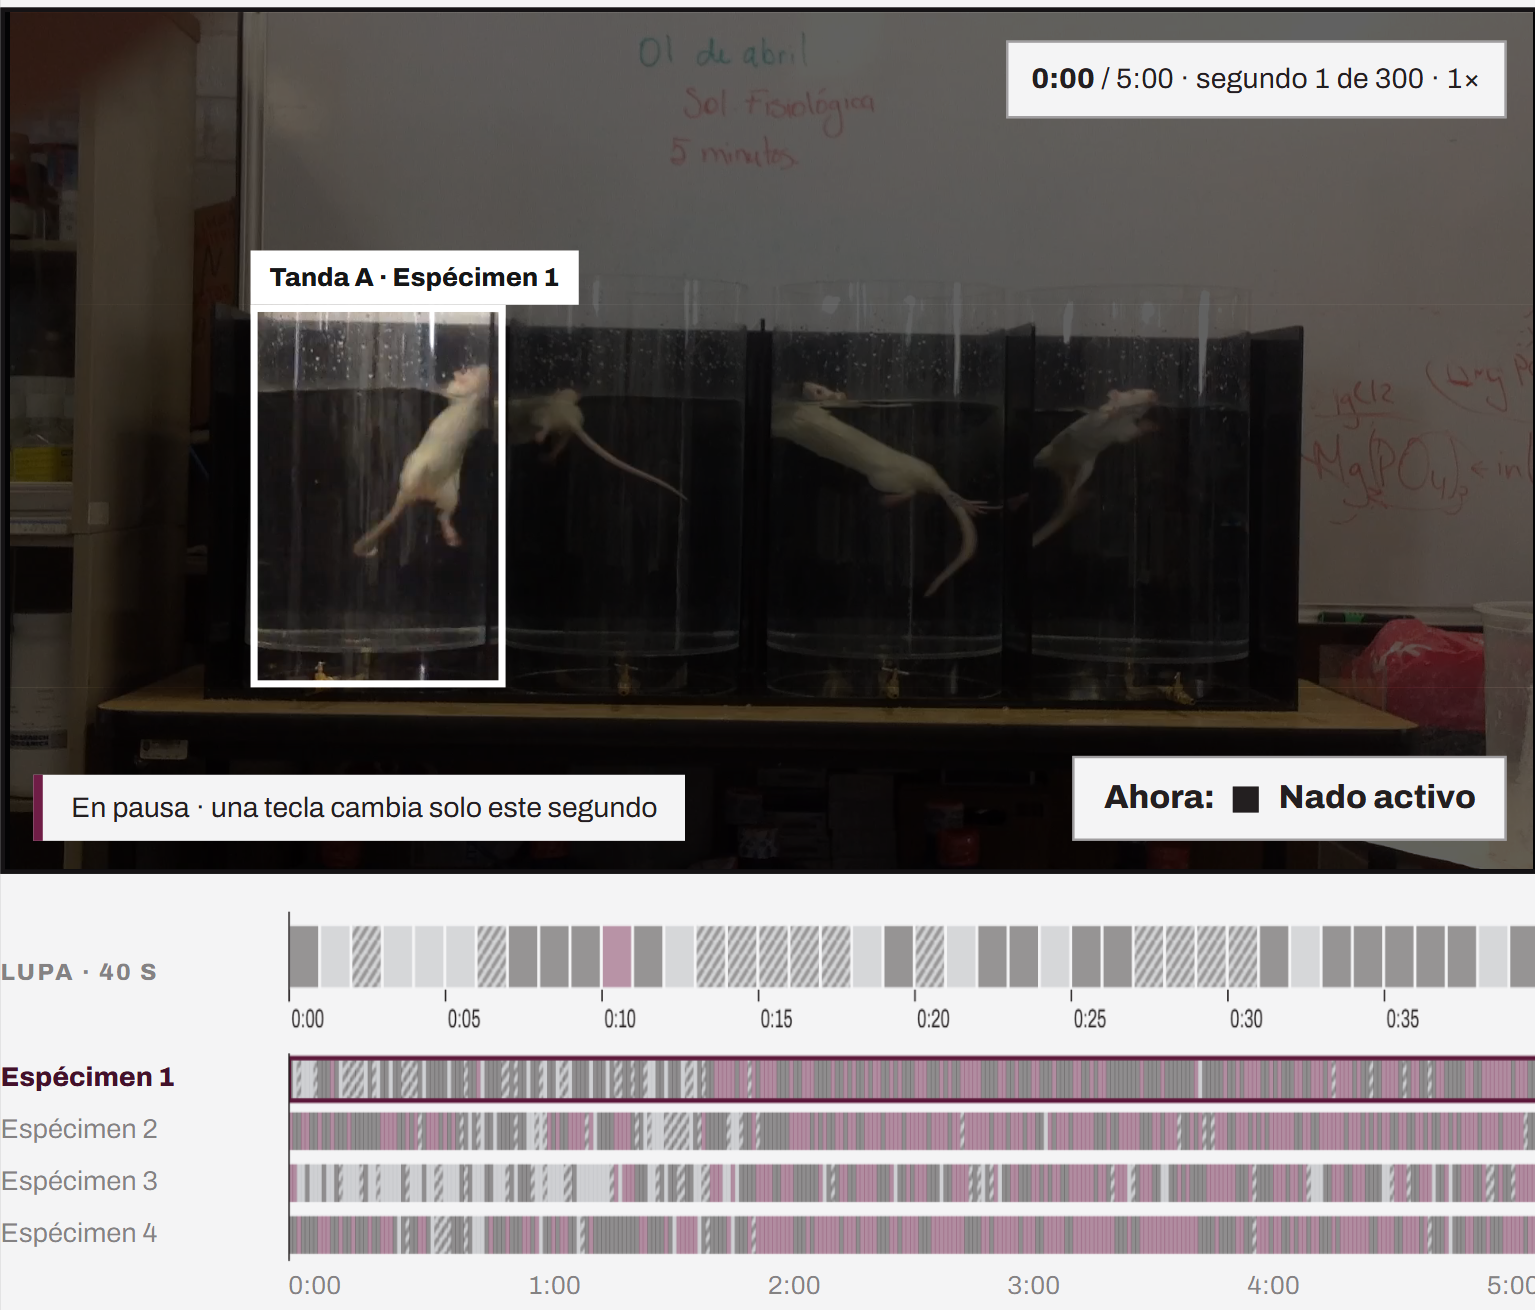
\includegraphics[width=\columnwidth]{figuras/revision.png}
\caption{Revisión segundo a segundo de un video real: recuadro del espécimen, conducta
actual, acercamiento de 40~s y líneas de conducta de los cuatro especímenes.}
\label{fig:revision}
\end{figure}

% =================================================================
\section{Resultados}

\subsection{Desempeño del clasificador}

Con la validación por video, el clasificador acertó en 71.6\% de los 7\,987 segundos
calificados, frente a 47.8\% de un sistema que contestara siempre «nado». Por bloques de
5~s la exactitud fue de 69.9\% sobre 1\,400 bloques completos. El F1 promedio fue de 0.705
(Tabla~\ref{tab:metricas}).

\begin{table}[t]
\renewcommand{\arraystretch}{1.15}
\caption{Desempeño por conducta en la validación por video}
\label{tab:metricas}
\centering
\footnotesize
\begin{tabular}{|l|c|c|c|r|}
\hline
\textbf{Conducta} & \textbf{Precisión} & \textbf{\textit{Recall}} & \textbf{F1} & \textbf{Segundos} \\
\hline
Escalamiento & 0.646 & 0.682 & 0.663 & 1\,244 \\
\hline
Inmovilidad & 0.727 & 0.710 & 0.719 & 2\,924 \\
\hline
Nado & 0.732 & 0.732 & 0.732 & 3\,819 \\
\hline
\textbf{Promedio} & & & \textbf{0.705} & 7\,987 \\
\hline
\end{tabular}
\end{table}

La matriz de confusión (Tabla~\ref{tab:confusion}) muestra que los errores más frecuentes
ocurren entre inmovilidad y nado (715 segundos en un sentido y 690 en el otro) y entre
escalamiento y nado (307 y 333). La inmovilidad casi no se confunde con el escalamiento.

\begin{table}[t]
\renewcommand{\arraystretch}{1.15}
\caption{Matriz de confusión, en segundos}
\label{tab:confusion}
\centering
\footnotesize
\begin{tabular}{|l|r|r|r|}
\hline
 & \multicolumn{3}{c|}{\textbf{Decidido por el clasificador}} \\
\cline{2-4}
\textbf{Marcado por el equipo} & \textbf{Escal.} & \textbf{Inmov.} & \textbf{Nado} \\
\hline
Escalamiento & \textbf{848} & 89 & 307 \\
\hline
Inmovilidad & 132 & \textbf{2\,077} & 715 \\
\hline
Nado & 333 & 690 & \textbf{2\,796} \\
\hline
\end{tabular}
\end{table}

Al separar solo inmovilidad de conducta activa, sobre los 8\,248 segundos, la exactitud fue
de 79.2\%, con F1 de 0.839 para la conducta activa y de 0.704 para la inmovilidad. La
confianza de la red es informativa: en los segundos con confianza de 0.8 o más (75\% del
total) la exactitud subió a 77.4\%, y con 0.9 o más (57\%), a 81.3\%.

\subsection{Pruebas del sistema}

El sistema cuenta con 739 pruebas automáticas: 278 del \textit{backend}, 93 del
\textit{worker} y 368 de la interfaz. Las 278 del \textit{backend}, ejecutadas con una base
PostgreSQL de pruebas, terminan sin fallos ni errores (una se omite por configuración) e
incluyen las restricciones de la base de datos. La Tabla~\ref{tab:sistema} resume la prueba de carga con
cuatro cuentas simultáneas y la verificación del sistema completo.

\begin{table}[t]
\renewcommand{\arraystretch}{1.15}
\caption{Prueba de carga y verificación del sistema completo}
\label{tab:sistema}
\centering
\footnotesize
\begin{tabular}{|l|l|}
\hline
\textbf{Medición} & \textbf{Resultado} \\
\hline
Peticiones en 120 s, cuatro cuentas & 1\,474, sin errores \\
\hline
Percentil 95 del tiempo de respuesta & 0.041 s \\
\hline
Respuesta más lenta (límite: 3 s) & 0.962 s \\
\hline
Video analizado & 301 s, 4 especímenes \\
\hline
Tiempo de análisis del sistema & Unos 9 min \\
\hline
Tiempo de anotación manual & Hasta unas 2 h \\
\hline
\end{tabular}
\end{table}

La verificación se hizo con el sistema armado a partir de sus imágenes y un video real del
segundo día. El análisis terminó sin intervención, lo que representa una reducción de más
del 90\% del tiempo; la revisión humana es opcional y se suma si se realiza. Esta prueba
confirma el funcionamiento de principio a fin, pero no mide el desempeño del clasificador.

\subsection{Limitaciones}

Los errores no son uniformes: cambian de un video a otro. En un espécimen el equipo marcó 47
segundos de escalamiento y el clasificador 117; en otro, 34 y 5. Además, 70\% de los bloques
de 5~s contiene más de una conducta, y el segundo de la transición es dudoso incluso para un
analista. El clasificador se entrenó y validó solo con la FST y con videos de un
laboratorio, y no se ha probado en otras condiciones de grabación. El sistema no corrige reflejos ni un contraste insuficiente, y no analiza el video del primer día. Por ello las cifras
deben leerse junto con la revisión segundo a segundo.

\subsection{Discusión}

Las cifras no se pueden comparar de forma directa con las de trabajos previos. DSAAN
\cite{dsaan} y la red 3D \cite{dellavalle} se validaron en condiciones controladas,
mientras que los videos de este laboratorio se graban con cámara web, tienen variaciones de
iluminación y muestran especímenes de pelaje claro con poco contraste; además, aquí cada
video se evalúa con una red que no lo vio durante el entrenamiento. La aportación está en
reunir, en un sistema instalable, la clasificación por segundo de las tres conductas, la
revisión humana y los reportes de cada experimento.

% =================================================================
\section{Conclusiones}

Se construyó un prototipo de sistema web que automatiza el análisis de videos de la prueba
de nado forzado, desde la carga hasta los reportes. El clasificador distingue por segundo
las tres conductas, con F1 entre 0.663 y 0.732, y separa la inmovilidad de la conducta
activa con una exactitud de 79.2\%. Un video de cuatro especímenes que requería hasta unas
dos horas de anotación se procesa en unos 9 minutos, con los mismos criterios en cada
análisis.

El sistema no sustituye el criterio del investigador: entrega una propuesta por segundo que
el laboratorio revisa y corrige. Al reunir los resultados y reportes de cada experimento en
un solo lugar, los deja consultables y libera horas
de anotación para diseñar e
interpretar experimentos, lo que puede favorecer la evaluación de más compuestos y dosis.

Como trabajo futuro se propone ampliar el sistema a otras pruebas conductuales, como el
laberinto en cruz elevado y el campo abierto; agregar medidas como la latencia a la primera
inmovilidad, los episodios por conducta y las comparaciones estadísticas entre grupos;
mejorar la robustez ante reflejos y bajo contraste; permitir el reentrenamiento desde el
sistema, y analizar la conducta en tiempo real.

% =================================================================
\section*{Reconocimientos}

Los autores agradecen al Instituto Politécnico Nacional y a la Escuela Superior de Cómputo
por las facilidades otorgadas, y al Laboratorio de Bioquímica Estructural, Sección de
Posgrado de la ENMyH, por los videos y la información del protocolo experimental.

% =================================================================
\IEEEtriggeratref{8}
\begin{thebibliography}{99}

\bibitem{who} World Health Organization, «Trastorno depresivo (depresión),» 2025. [En
línea]. Disponible: \url{https://www.who.int/es/news-room/fact-sheets/detail/depression}

\bibitem{porsolt} R.~D. Porsolt, M. Le~Pichon y M. Jalfre, «Depression: a new animal model
sensitive to antidepressant treatments,» \textit{Nature}, vol. 266, no. 5604, pp. 730--732,
1977.

\bibitem{dellavalle} A. Della~Valle et al., «Machine learning-based model for behavioural
analysis in rodents applied to the forced swim test,» \textit{Sci. Rep.}, vol. 15, no. 1,
art. 22314, 2025.

\bibitem{armario} A. Armario, «The forced swim test: Historical, conceptual and
methodological considerations and its relationship with individual behavioral traits,»
\textit{Neurosci. Biobehav. Rev.}, vol. 128, pp. 74--86, 2021.

\bibitem{slattery} D.~A. Slattery y J.~F. Cryan, «Using the rat forced swim test to assess
antidepressant-like activity in rodents,» \textit{Nat. Protoc.}, vol. 7, no. 6,
pp. 1009--1014, 2012.

\bibitem{detke} M.~J. Detke, M. Rickels e I. Lucki, «Active behaviors in the rat forced
swimming test differentially produced by serotonergic and noradrenergic antidepressants,»
\textit{Psychopharmacology}, vol. 121, no. 1, pp. 66--72, 1995.

\bibitem{nom} Secretaría de Agricultura, Ganadería, Desarrollo Rural, Pesca y Alimentación,
«NOM-062-ZOO-1999: Especificaciones técnicas para la producción, cuidado y uso de los
animales de laboratorio,» \textit{Diario Oficial de la Federación}, 2001.

\bibitem{ethovision} Noldus Information Technology, «EthoVision XT: Video tracking
software.» [En línea]. Disponible: \url{https://noldus.com/ethovision-xt}

\bibitem{anymaze} Stoelting Co., «ANY-maze: Video tracking software.» [En línea].
Disponible: \url{https://www.anymaze.com}

\bibitem{eztrack} Z.~T. Pennington et al., «ezTrack: An open-source video analysis pipeline
for the investigation of animal behavior,» \textit{Sci. Rep.}, vol. 9, no. 1, art. 19979,
2019.

\bibitem{dbscorer} A. Nandi, G. Virmani, A. Barve y S. Marathe, «DBscorer: An open-source
software for automated accurate analysis of rodent behavior in forced swim test and tail
suspension test,» \textit{eNeuro}, vol. 8, no. 6, 2021.

\bibitem{dsaan} X. Meng et al., «A deep-learning-based threshold-free method for automated
analysis of rodent behavior in the forced swim test and tail suspension test,» \textit{J.
Neurosci. Methods}, vol. 409, art. 110212, 2024.

\bibitem{sturman} O. Sturman et al., «Deep learning-based behavioral analysis enables high
precision rodent tracking and is capable of outperforming commercial solutions,»
\textit{Neuropsychopharmacology}, vol. 45, no. 11, pp. 1942--1952, 2020.

\bibitem{iso25010} ISO/IEC 25010:2011, \textit{Systems and software engineering --- SQuaRE
--- System and software quality models}, 2011.

\bibitem{iso12207} ISO/IEC/IEEE 12207:2017, \textit{Systems and software engineering ---
Software life cycle processes}, 2017.

\bibitem{piccardi} M. Piccardi, «Background subtraction techniques: a review,» en
\textit{Proc. IEEE Int. Conf. Systems, Man and Cybernetics}, 2004, pp. 3099--3104.

\bibitem{tran} D. Tran, H. Wang, L. Torresani, J. Ray, Y. LeCun y M. Paluri, «A closer look
at spatiotemporal convolutions for action recognition,» en \textit{Proc. IEEE Conf. Computer
Vision and Pattern Recognition (CVPR)}, 2018, pp. 6450--6459.

\bibitem{craft} R.~M. Craft, M.~L. Kostick, J.~A. Rogers, C.~L. White y K.~T. Tsutsui,
«Forced swim test behavior in postpartum rats,» \textit{Pharmacol. Biochem. Behav.},
vol. 96, no. 4, pp. 402--412, 2010.

\end{thebibliography}

\end{document}
